\chapter{Quantum machine learning with VQAs}
\label{chap:qml}

\section{Introduction}

Every discipline in computer science tries to gain some advantage from the usage of quantum computation, or establish whether there is any. Machine learning is no exception. The topic of quantum machine learning has considerable overlap with variational quantum algorithms, which motivates some attention to the topic within this thesis. In this chapter, we will mostly focus on quantum neural networks (QNN) rather than the more general techniques for quantum machine learning. The reason for that, as we shall soon see, is that modern QNNs can be essentially considered equivalent to variational circuits, and training quantum neural networks can be classified as a variational quantum algorithm. For broader reveiws, we refer the reader to Refs. \cite{schuld_introduction_2015,biamonte_quantum_2017, ciliberto_quantum_2018}.
% This is a rather narrow focus, we will first need to introduce the required supporting notions.

\subsection{Quantum neural networks}
 
What is a QNN? There is a multitude of ways one can come up with quantum analogues of a neural network. To do that, one needs to identify the key properties of a neural network that should be replicated. For example:

\begin{enumerate}
\item The network should consist of individual neurons connected to each other in a nontrivial manner, with tunable connection weights
\item The neurons should implement some kind of nonlinear activation functions.
\item The network is trained to solve its task by minimizing an error measured on the training samples.
\end{enumerate}


A big challenge in designing a quantum neural network is that all evolution that happens in quantum mechanins is linear, except for the measurement part, while classical neural networks are unthinkable without nonlinearity. 

\paragraph{Early QNN proposals.}
Here we will go in roughly chronological order. The first speculations about quantum neural computation can be found in Ref.~\cite{kak_quantum_1995}, but these only outline the concept without being too specific about the implementation. Behrman et al.~\cite{behrman_simulations_2000} proposed a neural network based on the interaction of quantum dots. Another proposal introduces nonlinearity through a dissipative, non-unitary operator \cite{gupta_quantum_2001}.

Some of these proposals can be summarized as follows. A quantum neuron (called `quron' in Ref.~\cite{schuld_quest_2014}) is a two-level quantum system, and different architectures engineer different interactions between the neurons. Such networks were reviewed by Schuld et al.~\cite{schuld_quest_2014}. It was observed that none of these networks can replicate the behavior of a Hopfield network -- a network which exhibits multiple stable states of its neurons. In a Hopfield network, the state of the neurons is iteratively updated based on the previous states and inter-neuron weights. Its key feature is that it has stable states and that the basins of attraction split all the state space, which is impossible if the evolution of a neural network is purely unitary.

\paragraph{Variational QNNs.}

The idea to use a generic variational circuit as a trainable model for a classification problem was independently proposed by Schuld et al.~\cite{schuld_circuit-centric_2020} and by Havlicek et al.~\cite{havlicek_supervised_2019}. The algorithm presented by us in Ref.~\cite{uvarov_machine_2020} and expanded upon in this chapter also belongs to this family. It is of course quite simple to implement feedforward networks in this setup, but one can also go for more complicated constructions, such as recurrent neural networks \cite{bausch_recurrent_2020}, generative adversarial networks \cite{dallaire-demers_quantum_2018} or convolutional neural networks \cite{pesah_absence_2020}.

While some QNNs of that kind do not even have well-defined neurons at this stage, others do define neurons as quantum gates that have several input qubits and one output qubit (possibly with ancilla qubits used in the process) \cite{cao_quantum_2017,bausch_recurrent_2020}. In this fashion, one can talk about layers in a QNN, which is somewhat more specific than layers in a general variational ansatz. Every unitary in the layer acts on all input qubits plus one output qubit. After all unitaries of that layer are applied, the output qubits are treated as input qubits for the next layer. Finally, the output qubits are measured after the last layer. Note that in this architecture, the input qubits from the last layer can be discarded and reused. This way, one can make deep quantum neural networks \cite{beer_training_2020} even with a limited budget of qubits, provided that the quantum processor can reinitialize qubits in runtime. 

\subsection{Quantum machine learning models viewed as kernel models}

An alternative view on the variational QNNs was presented in Ref.~\cite{schuld_quantum_2021}. Recall that our classifier circuit consists of two sub-circuit: one prepares the desired quantum state, another performs the classification. For a more general setup, the first part can be seen as an encoding circuit that maps classical data to quantum states. Let $x_i \in \mathcal{X} = \mathbb{R}^m$ be a classical data point with label $y_i \in \mathbb{R}$. Let us denote the corresponding quantum state $\ket{\phi(x_i)}$. Its density matrix is equal to $\rho(x_i) = \ket{\phi(x_i)}\bra{\phi(x_i)}$. When we prepare the state, apply the classifier circuit, and measure some observable $M$, we extract a prediction $\hat{y}_i \in \mathbb{R}$. The combination of a classifier circuit and a measurement is a function $f: \operatorname{Pos}(2^n) \rightarrow \mathbb{R}$:
\begin{equation}
    f(x) = \Tr(\rho(x) U^\dagger_{\mathrm{class}} (\boldsymbol{\varphi}) M U_{\mathrm{class}} (\boldsymbol{\varphi})).
\end{equation}
Here $\operatorname{Pos}(2^n)$ is the space of $2^n \times 2^n$ density matrices. Importantly, this function is linear in $\rho$, i.e.~$f$ belongs to the dual space. If the vector space has a basis (in our case, the basis of density matrices $\{\rho_i\}$) in with a fixed inner product (here we have $(a, b) = \Tr(a^\dagger b)$), then there is a natural choice of the dual basis: $\rho_i^* = (\rho_i, \placeholder)$.

Let us now introduce kernel models. A \textit{kernel} is a function $\kappa: \mathcal{X} \times  \mathcal{X} \rightarrow \mathbb{R}$. We require that this function takes larger values when its arguments are close to each other. Sometimes $\kappa$ is called a similarity function. Typically, $\kappa$ is also symmetric ($\kappa(x, x') = \kappa(x', x)$) and positive definite, that is, for all integer $l$ $x_1, .., x_l \in \mc{X}$, and any $c_1, ..., c_l \in \mathbb{R}$, the following is true \cite{vert_primer_2004}:
\begin{equation}
    \sum_{i=1}^l  \sum_{j=1}^l c_i c_j \kappa(x_i, x_j) \geq 0.
\end{equation}
Returning to the quantum models, we can choose a kernel as the inner product of the data points encoded in the state space:
\begin{equation}
    \kappa(x, x') = \Tr(\rho(x) \rho(x')).
\end{equation}

A famous result in the kernel theory, called the \textit{representer theorem}, states that any function minimizing the expected loss over the data set is expressed as a linear combination of kernel functions involving the data points:

\begin{equation}
    f_{\text{opt}}(x) = \sum_i \alpha_i \kappa(x_i, x), \quad \quad \alpha_i \in \mathbb{R}
\end{equation}

Moreover, in this form, the optimization of the coefficients is \textit{convex}. This means that in principle, one can replace the QNNs with kernel models of that kind and always find a global optimum. On the other hand, for a data set with $m$ points, one will need to estimate $O(m^2)$ inner products, and the classification of a data point will take $O(m)$ evaluations. For big data applications, this is a disadvantage compared to QNNs. For instance, the classification of a data point for a QNN takes $O(1)$ in the number of data points, while training can sometimes take less than $O(m^2)$.

% It was later observed that such networks are essentially kernel models, except that the kernel is now more complicated to evaluate, and that's where the advantage may come from.

% \subsection{Encoding classical data to a quantum computer}

% In order to do something with the data, a quantum computer must receive it as quantum states. There are different encodings which lead to different results.

% \section{Selected theoretical results on QML}

An interesting question is whether a quantum ML model bring any advantage in predicting the outcomes of quantum experiments. Huang and coworkers \cite{huang_information-theoretic_2021} show that, in a very general setting, a quantum ML model does not bring any advantage in terms of average-case error, but does bring exponential advantage in terms of worst-case error.

\section{Quantum classifier to partition quantum data}

\paragraph{Learning the phase of the transverse-field Ising model. } Here we demonstrate how we solve a machine learning problem that is intrinsically quantum. Recall that in chapter \ref{chap:vqe_numerics} we studied the transverse field Ising model:

\begin{equation}
\label{eq:tfim_2}
    H = J \sum Z_i Z_{i+1} + h \sum X_i.
\end{equation}

This model has a known phase transition at $J=h$. Using this fact, we set up our machine learning problem as follows:

\begin{itemize}
    \item The data points are the approximate ground states of (\ref{eq:tfim_2}) for $J=1$ and different values of $h$. The approximate states none other than the VQE solutions. We took the best set of solutions we had in terms of energy error --- the one found using four layers of the checkerboard ansatz.
    \item Given a quantum state, promised to be a ground state of the TFI model, the task is to tell whether $h<1$ or $h>1$ for this state.
\end{itemize}

To solve this problem, we employ a variational ansatz. Let $U_{\mathrm{VQE}}(\boldsymbol{\theta})$ be the ansatz that prepares the input state $\ket{\psi(\boldsymbol{\theta})}$ that is to be classified. Denote $U_{\mathrm{class}}(\boldsymbol{\varphi})$ the classifier unitary. Then, to evaluate the class of $\ket{\psi(\boldsymbol{\theta})}$, we prepare $U_{\mathrm{class}}(\boldsymbol{\varphi}) \ket{\psi(\boldsymbol{\theta})}$, measure all qubits, and decide the class by majority of the qubits. The quantum circuit is schematically shown in Fig.~\ref{fig:classifier_scheme}. For the transverse-field Ising model, the classifier circuit $U_{\mathrm{class}}(\boldsymbol{\varphi})$ had the same depth as the VQE circuit (i.e.~four layers of the checkerboard ansatz).

Effectively, estimating the majority is equivalent to estimating the energy of the state $U_{\mathrm{class}}(\boldsymbol{\varphi}) \ket{\psi(\boldsymbol{\theta})}$ relative to the following Hamiltonian:
\begin{equation}
    \label{eq:h_vote}
    H_{\text{vote}} = \sum_{w(i) > n/2} \ket{i} \bra{i} + \frac{1}{2}\sum_{w(i) = n/2} \ket{i} \bra{i}.
\end{equation}
Here $w(i)$ denotes the Hamming weight of the basis state $\ket{i}$, i.e.~the number of ones it contains.

%%It would be a bad idea to use parity as the signal because of BPs, right? Here the situation is less obvious: we have nonlocal projectors, but there is an exponential number of these so it's not that bad actually.

\begin{figure}
    \centering
    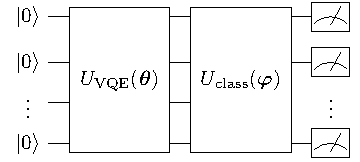
\includegraphics[width=0.7\linewidth]{figures/classifier_circuit.pdf}
    \caption{Quantum circuit that implements the classifier. The first part prepares the VQE solution, the second one performs the classification. The assigned label is inferred from the measurements in the $Z$ basis. Both $U_{\mathrm{VQE}}$ and $U_{\mathrm{class}}$ have the checkerboard structure. Reprinted from \cite{uvarov_machine_2020}.}
    \label{fig:classifier_scheme}
\end{figure}

To train the classifier circuit $U_{\mathrm{class}}(\boldsymbol{\varphi})$, we used the log-likelihood cost function. Let $\{ (\boldsymbol{\theta}_i, y_i) \}_{i=1}^{N_{train}}$ be the set of training data points and their labels, $y_i \in \{0, 1\}$. Let $p_i \in [0, 1]$ be the label predicted by the neural network:
\begin{equation}
    p_i = \bra{\psi(\boldsymbol{\theta}_i)} U^\dagger_{\mathrm{class}} (\boldsymbol{\varphi})H_{\text{vote}} U_{\mathrm{class}}(\boldsymbol{\varphi})\ket{\psi(\boldsymbol{\theta}_i)}.
\end{equation}
Then the loss function is:
\begin{equation}
\label{eq:logloss}
    f = -\sum_{i=1}^{N_{train}} \left( y_i \log p_i + (1 - y_i) \log (1 - p_i) \right).
\end{equation}

To minimize $f$, we used the simultaneous perturbation stochastic approximation (SPSA) algorithm \cite{spall_multivariate_1992}. This algorithm estimates the gradient vector by computing a finite difference in random direction, then performs a gradient descent step. We optimized the log loss over 300 epochs, with both finite differences step size and learning rate starting very coarse and decreasing as $1/\sqrt{n_{epoch}}$, where $n_{epoch}$ is the epoch number.

The result of the classification is shown in Fig.~\ref{fig:phase_classification}, left. The horizontal axis depicts the true value of $h$, while the vertical axis shows the label predicted by the classifier. In this case, the classification problem was quite simple, yielding a high accuracy score (97\%). The TFI model, however, can be easily partitioned without any machine learning: the value of total magnetization along the $X$ axis is also a good predictor of the phase of the system: with the increase of $h$, the magnetization gradually increases and cusps around the phase transition point (see Fig. \ref{fig:x_classifies_phases}). For this reason, we also performed the same analysis for a more complicated model.

\begin{figure}
    \centering
    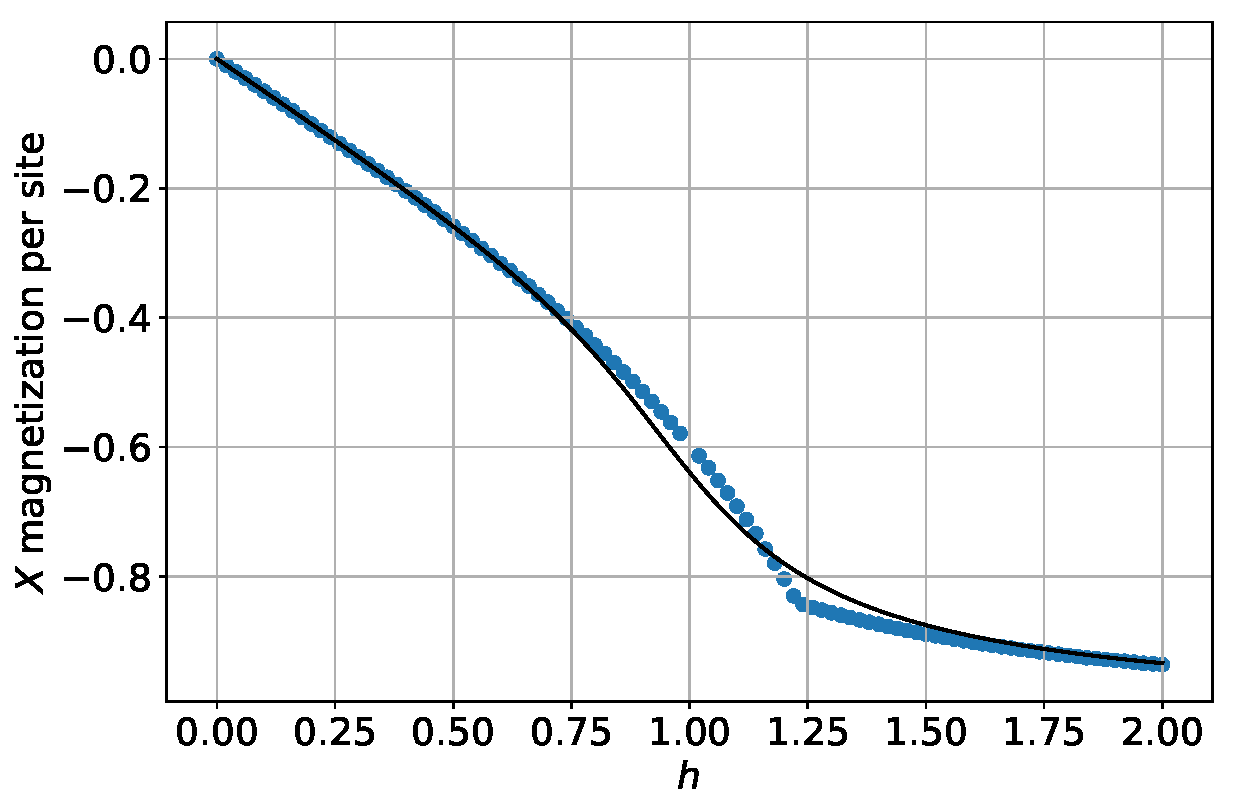
\includegraphics[width=0.7\linewidth]{figures/x_classifies_tfim.pdf}
    \caption{Total magnetization of the ground state as a function of the transverse field $h$. Solid line: exact ground states, markers: VQE solutions.}
    \label{fig:x_classifies_phases}
\end{figure}


\paragraph{Heisenberg $XXZ$ model.} Recall that the Heisenberg $XXZ$ model is described by the following Hamiltonian (\ref{eq:heisenberg_xxz}):

\begin{equation}
H = \sum_{i=1}^n \left[J_\perp\left(X_i X_{i+1} + Y_i Y_{i+1}\right)
    + J_z Z_i Z_{i+1}\right].
\end{equation}

From a physical perspective, Eq.~(\ref{eq:heisenberg_xxz}) corresponds to a uniform exchange coupled system with a uniaxial anisotropy specified by $J_z$. At $|J_z| < J_\perp$, this model is in the XY, or planar, phase which is characterized by algebraic decay of equal-time spin-spin correlation functions. In the regime $J_z > J_\perp$ the Hamiltonian corresponds to the antiferromagnetic Ising state. The system undergoes a Berezinsky--Kosterlitz--Thouless type phase transition at $J_z = J_\perp$   \cite{franchini_introduction_2017}. At the phase transition point, the ground state has the highest nearest-neighbour concurrence and a cusp in nearest-neighbour quantum discord \cite{dillenschneider_quantum_2008}.

For this model, there is some rotational symmetry that preserves the energy of the state. Namely, $H$ commutes with the operator of rotating each qubit around the $Z$ axis by an angle $\varphi$. In addition, $H$ commutes with all-qubit spin flip operators $X^{\otimes n}$ and $Z^{\otimes n}$. This enables us to perform a procedure of data augmentation by applying these operators to the approximate ground states. The new states obtained this way will be just as good in terms of the energy error. Recall that the ansatz we used consists of two-qubit entangler gates shown in Fig. \ref{fig:entangler}:
\begin{equation*}
    \mbox{
        \Qcircuit @C=1.0em @R=1.0em {
               & \gate{e^{-i \tilde{\theta}_1 X}} & \multigate{1}{e^{-i \tilde{\theta}_3 {Z} \otimes {Z}}} & \gate{e^{-i \tilde{\theta}_4 Z}} & \qw \\
               & \gate{e^{-i \tilde{\theta}_2 X}} & \ghost{e^{-i \tilde{\theta}_3 Z \otimes Z}} & \gate{e^{-i \tilde{\theta}_5 Z}} & \qw \\
           }
        }
\end{equation*}
The $Z$ rotation to all qubits can easily be applied by increasing all angles in the last layer of the operators by $\varphi$. The $X$ flip can be performed by inverting the angles of the $Z$ rotations in the last layer (because $Z$ and $X$ anticommute) and increasing the angles of the $X$ rotations by $\pi / 2$. Note that the rotation gates are often written with the angle divided by half, e.g.~$R_y = \exp(-\rmi \frac{\theta}{2} Y)$. In this case, the parameters should instead be incremented by $\pi$.


The result is depicted in in Fig.~\ref{fig:phase_classification}, right. Compared to the TFI model, we had to increase the depth of the classifier circuit to 6 layers. The resulting plot is much more jagged, and the accuracy is somewhat lower (93\%). The reason for the points being spread around is likely the data augmentation procedure. However, without data augmentation, the data points do not represent the state space accurately. The reason for that is the usage of AAVQE, which forces the solution points for neighboring values of $h$ to be close to each other, despite the freedom granted by the rotational symmetry.


\begin{figure}
    % \centering
    % 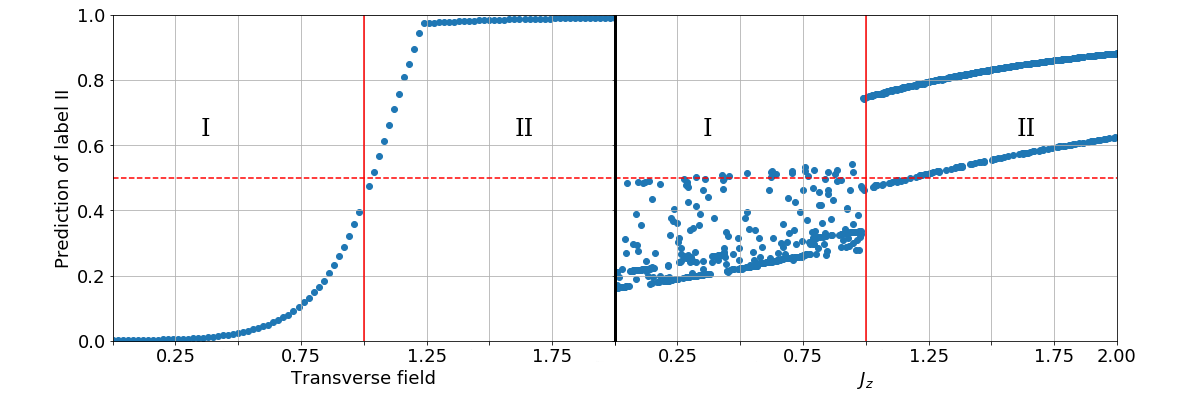
\includegraphics[width=0.9\linewidth]{figures/merged.png}
    \centering
    \begin{subfigure}{.48\linewidth}
        \centering
        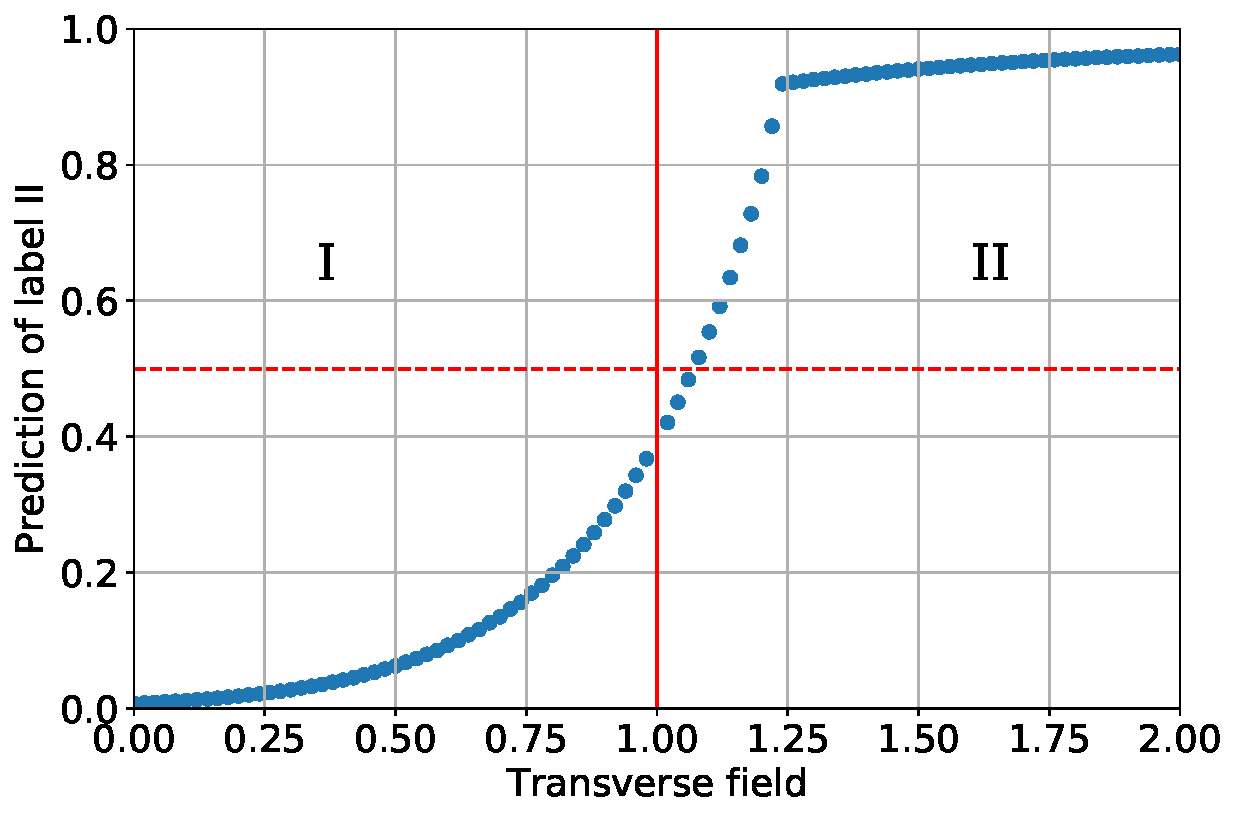
\includegraphics[width=\textwidth]{figures/tfi_classification_new_2021}
    \end{subfigure}\begin{subfigure}{.48\linewidth}
        \centering
        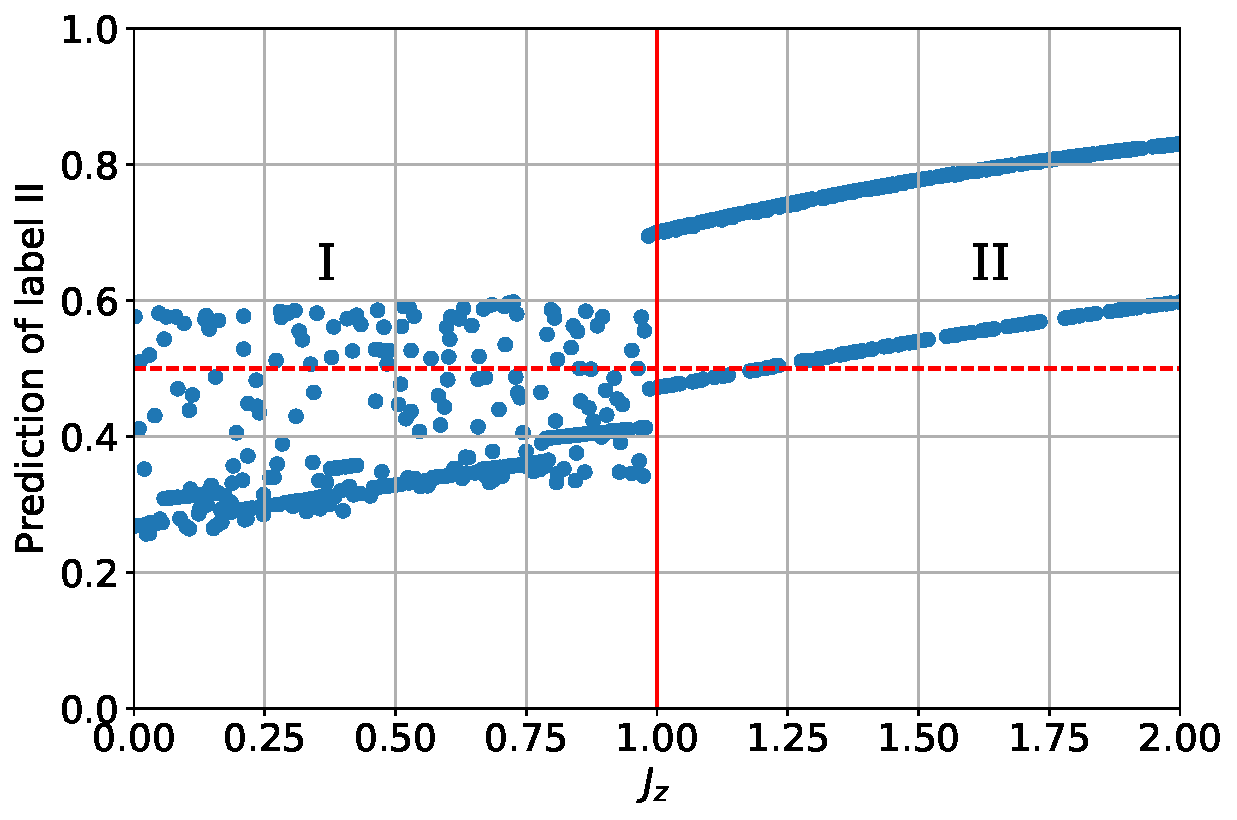
\includegraphics[width=\textwidth]{figures/xxz_classification_new_2021.pdf}
    \end{subfigure}
    \caption{Left: predicted label of phase II as a function of magnetic field for transverse field Ising model. Right: predicted label of phase II as a function of $J_z$ for the XXZ model. Roman numbers denote the phases I and II of the models.}
    \label{fig:phase_classification}
\end{figure}
% Not reprinted from Uvarov et al PRA 2020 because these are slightly different figures

\paragraph{Random Hamiltonians.} Simpler toy models, like the TFI model, may have simple classification criteria which do not require application of machine learning. Here we classify the solutions of a randomized model: $H(\alpha) = (1 - \alpha) H_1 + \alpha H_2, \ \alpha \in [0, 1]$, where $H_1$ and $H_2$ are random Hermitian matrices sampled from the Gaussian unitary ensemble. We split solutions in two classes: (i) $\alpha < 0.5$ and (ii) $\alpha > 0.5$. Then we run the optimization routine to train the learning circuit to discern between the two classes. 

The approach was tested for 6 qubits, $n=100$, where $n_\text{train} = 70$, $n_{\text{test}} = 30$. The depth of the VQE circuit and the classifier were both set to four layers. The results are shown in Fig.~\ref{fig:learning_random_hams}. For this configuration, the accuracy of $93 \%$ was reached. This shows that the algorithm works even for a problem where there are no simple physically-motivated criteria. Naturally, having some structure compatible with the circuit topology would greatly benefit the convergence for larger problems.


\begin{figure}
    \centering
    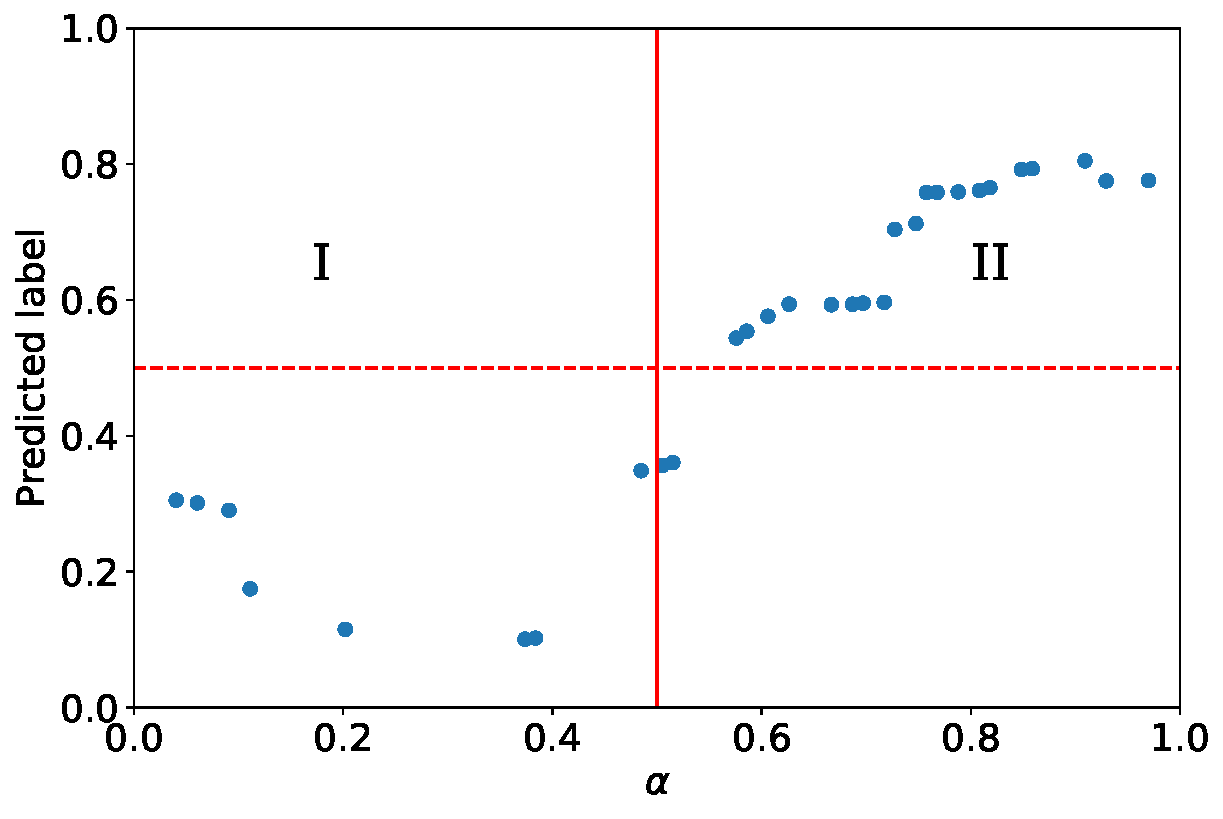
\includegraphics[width=0.7\linewidth]{figures/learning_random_hams}
    \caption{Results of learning on the random Hamiltonians model. Roman letters denote label classes. Reprinted from \cite{uvarov_machine_2020}.}
    \label{fig:learning_random_hams}
\end{figure}

\section{Discussion}

\subsection{Learning by confusion}
In this example, we knew the location of the phase transition point all along. But what if the task is to actually locate this point? This is also possible. The idea is as follows: let us pick a random value $h^*$, partition the data points across this point, and train the classifier. If the value $h^*$ is very far from all data points, all points will belong to one class, and the classifier will be able to partition them with 100\% accuracy. If $h^*$ does split the data points nontrivially, but is in the wrong location, then some points will be very close, but in the different classes, which will lead to a suboptimal training accuracy. Finally, the accuracy will be maximal when $h^*$ is the correct value. This behavior was observed for a classical neural network learning on spin states \cite{van_nieuwenburg_learning_2017}.

We reproduced the same experiment for our quantum neural network for the task of classifying the ground states of the TFI model. The result is shown in Fig. \ref{fig:learning_by_confusion}. Surprisingly enough, even though the accuracy does peak around the correct value of $h$, the characteristic W-shaped curve seen in \cite{van_nieuwenburg_learning_2017} is not observed. 
% \todo{Same for the XXZ model?}

\begin{figure}
    \centering
    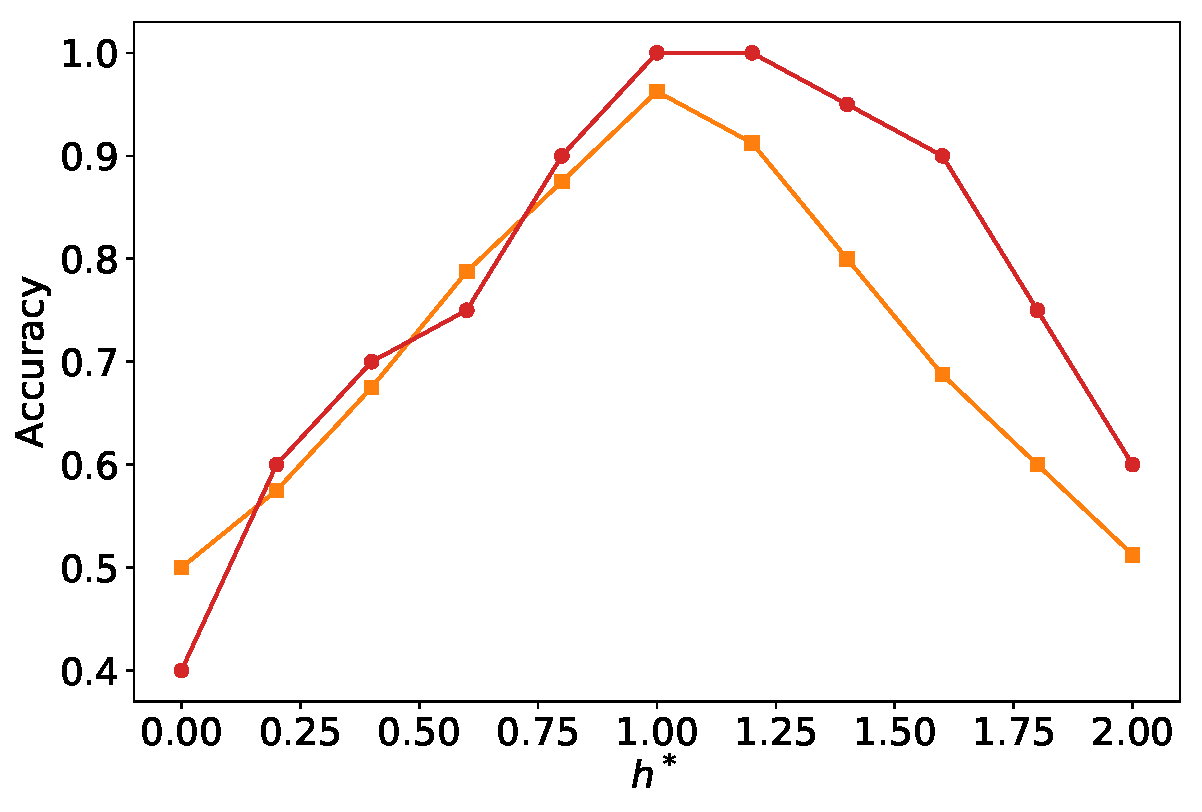
\includegraphics[width=0.7\linewidth]{figures/acc_confusion_2.pdf}
    \caption{Train (squares) and test (circles) accuracy of the classifier for data marked with proposed threshold $h^*$.}
    \label{fig:learning_by_confusion}
\end{figure}


\subsection{Possible choices for the labeling procedure}

The unitary classifier circuit $U_{\mathrm{class}}(\boldsymbol{\varphi})$ by itself takes an input state and produces an output state. Then the measurements translate them into a probability distribution on the values of the output bits. The choice how to translate this distribution into a final label also has substantial freedom. In the pioneering work on such classifiers \cite{schuld_circuit-centric_2020}, the authors simply measure the output of the first qubit. In this situation, the label is assigned by the following rule:

\begin{equation}
    p_i = \frac{1}{2}\bra{\psi(\boldsymbol{\theta}_i)} U^\dagger_{\mathrm{class}} (\boldsymbol{\varphi})(1 + Z_1) U_{\mathrm{class}}(\boldsymbol{\varphi})\ket{\psi(\boldsymbol{\theta}_i)}.
\end{equation}

While this is a straightforward option, it does introduce some asymmetry in the model, which can only recovered by a long classifier circuit. For example, for circuit of depth $O(1)$, most qubits (and hence most of the input data) would not affect the measurement outcome in any way. To deal with this asymmetry, we proposed the majority-vote classifier described earlier.

New evidence suggests that the choice of the method to translate measurement results into labels may affect the trainability of the circuit. Such a choice can be translated to a Hamiltonian, and the locality of the latter may induce the barren plateaus in the optimization landscape \cite{uvarov_barren_2021,cerezo_cost-function-dependent_2020}. This locality dependence will be studied in more detail in Chapter \ref{chap:plateaus}. Still, the majority vote classifier is not necessarily a bad choice. It's true that the Hamiltonian $H_\text{vote}$ (\ref{eq:h_vote}) is highly non-local, but on the other hand it contains an exponential number of terms, which may offset the barren plateaus effect. Besides, since we count the number of ones in the output state, even flipping one qubit has a substantial effect on the output.

% \todo{In Skolik et al \cite{skolik_layerwise_2020}, the authors also measure just the first qubit. What does the effective Hamiltonian looks like for one layer of HEA? Also, if we grok that, we may understand when does layerwise learning actually help with BPs and such.}



\section{Conclusions}

In this chapter, we gave an overview of methods to transfer the idea of neural networks to quantum computing. We proposed and numerically implemented a quantum classifier and trained it on quantum states constructed by VQE. 
It is a nontrivial fact that the Ising model required fewer layers than the XXZ model. In the transverse field Ising model, the magnetization $\sum \langle \sigma_x^{(i)} \rangle$ as a function of magnetic field clearly points at the location of the phase transition points. This implies that the phases of the model are easy to classify. In the XXZ model, the transition at $J_z=1$ is a transition between a paramagnetic and an antiferromagnetic phase \cite{franchini_introduction_2017}. Neither of these phases shows spontaneous magnetic moment in absence of an external field, making it somewhat harder to discern the two phases. 
The proposed classification technique can be applied to any model that can be expressed as a spin model (e.g.~fermion problems can be mapped to spin problems by using Jordan--Wigner transformation or Bravyi--Kitaev transformation).

In addition, we recreated an experiment for learning by confusion \cite{van_nieuwenburg_learning_2017} in the quantum setup. We found that this technique does pinpoint the location of the phase transition, but the shape of the curve is substantially different from the classical. We hypothesize that in this situation the classifier just did not have enough expressive power to mark all states with the same label.

